{\scriptsize%
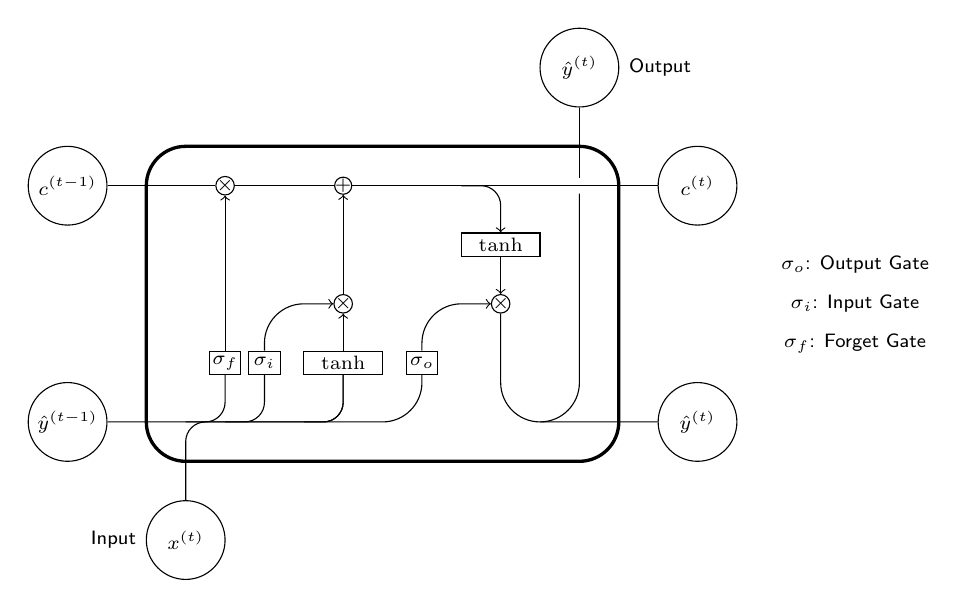
\begin{tikzpicture}[
    % GLOBAL CFG
    font=\sf \scriptsize,
    %>=LaTeX,
    % Styles
    cell/.style={% For the main box
        rectangle,
        rounded corners=5mm,
        draw,
        very thick,
        },
    operator/.style={%For operators like +  and  x
        circle,
        draw,
        inner sep=-0.5pt,
        minimum height =.2cm,
        },
    function/.style={%For functions
        ellipse,
        draw,
        inner sep=1pt
        },
    ct/.style={% For external inputs and outputs
        circle,
        draw,
        %line width = .75pt,
        minimum width=1cm,
        inner sep=1pt,
        },
    gt/.style={% For internal inputs
        rectangle,
        draw,
        minimum width=4mm,
        minimum height=3mm,
        inner sep=1pt
        },
    mylabel/.style={% something new that I have learned
        font=\scriptsize\sffamily
        },
    ArrowC1/.style={% Arrows with rounded corners
        rounded corners=.25cm,
        %thick,
        },
    ArrowC2/.style={% Arrows with big rounded corners
        rounded corners=.5cm,
        %thick,
        },
    ]

%Start drawing the thing...
    % Draw the cell:
    \node [cell, minimum height =4cm, minimum width=6cm] at (0,0){} ;

    % Draw inputs named ibox#
    \node [gt] (ibox1) at (-2,-0.75) {$\sigma_f$};
    % forget
    \node [gt] (ibox2) at (-1.5,-0.75) {$\sigma_i$};
    % input
    \node [gt, minimum width=1cm] (ibox3) at (-0.5,-0.75) {$\tanh$};
    \node [gt] (ibox4) at (0.5,-0.75) {$\sigma_o$};
    % output

   % Draw opérators   named mux# , add# and func#
    \node [operator] (mux1) at (-2,1.5) {$\times$};
    \node [operator] (add1) at (-0.5,1.5) {+};
    \node [operator] (mux2) at (-0.5,0) {$\times$};
    \node [operator] (mux3) at (1.5,0) {$\times$};
    \node [gt, minimum width=1cm] (func1) at (1.5,0.75) {$\tanh$};
    % memory cell

    % Draw External inputs? named as basis c,h,x
    \node[ct, label={[mylabel]}] (c) at (-4,1.5) {$c^{(t-1)}$};
    \node[ct, label={[mylabel]}] (h) at (-4,-1.5) {$\hat{y}^{(t-1)}$};
    \node[ct, label={[mylabel]left:Input}] (x) at (-2.5,-3) {$x^{(t)}$};

    % Draw External outputs? named as basis c2,h2,x2
    \node[ct, label={[mylabel]}] (c2) at (4,1.5) {$c^{(t)}$};
    \node[ct, label={[mylabel]}] (h2) at (4,-1.5) {$\hat{y}^{(t)}$};
    \node[ct, label={[mylabel]right:Output}] (x2) at (2.5,3) {$\hat{y}^{(t)}$};

    \node (fg) at (6,-0.5) {$\sigma_f$: Forget Gate};
    \node (ig) at (6,0) {$\sigma_i$: Input Gate};
    \node (og) at (6,0.5) {$\sigma_o$: Output Gate};

% Start connecting all.
    %Intersections and displacements are used.
    % Drawing arrows
    \draw [ArrowC1] (c) -- (mux1) -- (add1) -- (c2);

    % Inputs
    \draw [ArrowC2] (h) -| (ibox4);
    \draw [ArrowC1] (h -| ibox1)++(-0.5,0) -| (ibox1);
    \draw [ArrowC1] (h -| ibox2)++(-0.5,0) -| (ibox2);
    \draw [ArrowC1] (h -| ibox3)++(-0.5,0) -| (ibox3);
    \draw [ArrowC1] (x) -- (x |- h)-| (ibox3);

    % Internal
    \draw [->, ArrowC2] (ibox1) -- (mux1);
    \draw [->, ArrowC2] (ibox2) |- (mux2);
    \draw [->, ArrowC2] (ibox3) -- (mux2);
    \draw [->, ArrowC2] (ibox4) |- (mux3);
    \draw [->, ArrowC2] (mux2) -- (add1);
    \draw [->, ArrowC1] (add1 -| func1)++(-0.5,0) -| (func1);
    \draw [->, ArrowC2] (func1) -- (mux3);

    %Outputs
    \draw [-, ArrowC2] (mux3) |- (h2);
    \draw (c2 -| x2) ++(0,-0.1) coordinate (i1);
    \draw [-, ArrowC2] (h2 -| x2)++(-0.5,0) -| (i1);
    \draw [-, ArrowC2] (i1)++(0,0.2) -- (x2);
\end{tikzpicture}
}
